\documentclass[letterpaper]{article}

\usepackage{hyperref}
\usepackage{tikz}
\usepackage{listings}

\definecolor{code_green}{rgb}{0, 0.6, 0}

\lstdefinestyle{Code_Style}{
    basicstyle=\ttfamily,
    commentstyle=\color{code_green},
    keywordstyle=\color{blue},
    breakatwhitespace=false,
    breaklines=true,
    keepspaces=true,
    numbers=left,
    showspaces=false,                
    showstringspaces=false,
    showtabs=false,
    tabsize=4
}

\lstset{style=Code_Style}

\title{Amazon Delivery Truck Simulation}
\author{Hanna Butt \thanks{HFB352, \href{mailto:hannaf2020@gmail.com}{hannaf2020@gmail.com}} \and Ashton Cole \thanks{AVC687, \href{mailto:ashtonc24@utexas.edu}{ashtonc24@utexas.edu}} \and Kelechi Emeruwa \thanks{KEE688, \href{mailto:kelechi@utexas.edu}{kelechi@utexas.edu}}}
\date{\today}

\begin{document}
    \maketitle

    \begin{abstract}
        Summary of whole paper. Note that this is not an introduction or context, but a summary.
    \end{abstract}

    \section{Introduction}
    \label{section:Introduction}
    Imagine that a delivery company has a series of orders that it needs to fulfill. It has a truck that can stop at each address and make the delivery. The company naturally wants to save on time and fuel costs, so it tries to find the shortest path from its warehouse to cover all of the stops. This is the basic premise of the Traveling Salesman problem. Our team chose to solve for our final project in COE 322: Scientific Computation at the University of Texas at Austin for the fall of 2022.
    
    In Section \ref{section:Methodology} we discuss the algorithm that we used to solve the simple Traveling Salesman Problem, and expansions upon it to construct our final program. In Section \ref{section:Results}, we display the outcomes of several test scenarios and discuss the results. Finally, in Section \ref{section:Conclusion}, we offer our final thoughts and reflect on ethical considerations. However, we will first further define the problem for our purposes and apply some limitations and assumptions in the following subsections.

    \subsection{Perfect is the Enemy of Good}
    \label{subsection:Perfect_is_the_Enemy_of_Good}
    One could simply test each of the $n!$ combinations of a list of $n$ addresses to fund the one with the shortest total distance, but with 4 stops this becomes quite tedious, and after that nearly untenable. A computer could solve this faster, but the problem still becomes very computationally expensive at a factorial rate. The preferable alternative is to use algorithms to find good and better paths, significantly cutting down on calculations. Perhaps it will neglect the perfect solution, but in a world with finite resources, we have to make the trade-off to settle for less. The algorithms which we employ, detailed in Section \ref{section:Methodology} reflect this.

    \subsection{Eath is Flat}
    \label{subection:Earth_is_Flat}
    We also have to restrict the definitions of an address and the distance between addresses. Since this project is intended to focus on the algorithms one would use to solve the Traveling Salesman problem, as opposed to practical considerations for constructing a turn-key solution for use in the real world, addresses are represented with Cartesian coordinates on a two-dimensional Euclidian plane. Distances are assumed to be Euclidian, i.e. ``as the bird flies,'' and travel times are assumed to be proportional thereto. The distance could alternatively be defined as the ``Manhattan Distance,'' i.e. the distance in a perfect rectilinear street grid. Using real-world geographic data considering road layouts, speed limits, real-time traffic data, and Earth's curvature would be more realistic, but it would also add significant complexity to our implementation while contributing little to the core principles of the solution.

    \subsection{TODO}
    MORE DEFINITIONS HERE: deliver by date, multiple days, multiple trucks

    \section{Methodology}
    \label{section:Methodology}
    % Notes: Talk about how we're solving the problem (C++, TACC super computer, icpc compiler) and how the program works (e.g. reads in text file, spits out text file). Then go into the development process/timeline (we started simple with address/list classes, tested functionality, and then expand it a bit)

    To approach this problem, we wrote a library and scripts in C++. These were compiled with \verb|g++| on our local machines and \verb|icpc| on the Texas Advanced Computing Center's ISP supercomputer. These scripts are outlined below.
    \begin{itemize}
        \item \verb|traveling_salesman.h|: a header file for our TravelingSalesman library, defining all of the objects and algorithms used in the project
        \item \verb|traveling_salesman.cpp|: an implementation file
        \item \verb|tester.cpp|: a script which tests the functionality of our TravelingSalesman library and generates TikZ code for figures displayed in this report; this script is compiled as \verb|tester.exe|
        \item \verb|routeGenerator.cpp|: a script which generates \verb|.dat| files containing lists of orders to be processed by \verb|delivery_truck_simulation.exe|; this script is compiled as \verb|routeGenerator.exe|
        \item \verb|delivery_truck_simulation.cpp|: a script which represents a hypothetical final product for use in industry, as described in Section \ref{subsection:Developing_the_Final_Product}; this script is compiled as \verb|delivery_truck_simulation.exe|
    \end{itemize}

    We began our project by writing the header and implementation files, coupled with tests in our tester file. After we confirmed that all of our objects and algorithms functioned as expected, we designed a main program to best parallel a real world application of solving the Traveling Salesman Problem. The structures and algorithms that we developed are further detailed in this section.

    In Section \ref{subsection:Object-Oriented_Structure}, we outline the structure of the classes that we used to represent and solve the problem. In Section \ref{subsection:Traveling_Salesman_Problem}, we describe the algorithms we used to solve the simple Traveling Salesman Problem. In Section \ref{subsection:Multiple_Traveling_Salesmen_Problem}, we describe the expansion of the problem to account for optimizing multiple delivery routes. Finally, in Section \ref{subsection:Developing_the_Final_Product}, we describe how we combined our algorithms into a final product for a hypothetical user.

    \subsection{Object-Oriented Structure}
    \label{subsection:Object-Oriented_Structure}
    Our scripts took advantage of C++'s object-oriented capabilities to organize the problem. This section provides a brief overview; the contents of these classes are not described exhaustively.
    
    Each delivery stop is represented by an \verb|Address| object, which has two-dimensional integer Cartesian coordinates \verb|i| and \verb|j| representing the location of the address, an an integer \verb|deliver_by| which describes the day by which the order is supposed to be delivered. The class can also calculate the distance to other \verb|Address|es, using either the Euclidian distance $\sqrt{i^{2} + j^{2}}$ or Manhattan distance $|i| + |j|$. In our implementation, we use the Euclidian distance, but it could easily be replaced with another formula.

    A list of \verb|Address|es is represented by an \verb|AddressList| object, which holds the objects in a \verb|std::vector<Address>| instance variable called \verb|address_list|. This class can add, remove, and rearrange \verb|Address|es.

    The \verb|Route| class extends the \verb|AddressList| class by including a \verb|hub| instance of type \verb|Address|. This represents the starting and ending point of the \verb|Route|. This class contains several functions to solve variants of the Traveling Salesman problem.

    \subsection{Traveling Salesman Problem}
    \label{subsection:Traveling_Salesman_Problem}

    Talk about greedy and opt2 algorithms.

    \begin{figure}[h]
        \caption{An unsorted Route is optimized through both the greedy algorithm (blue) and the opt2 algorithm (green). This demonstrates how the opt2 algorithm alone is not necessarily sufficient to find the shortest Route.}
        \label{figure:sortdemo}
        \begin{minipage}{0.3\linewidth}
            % Old
            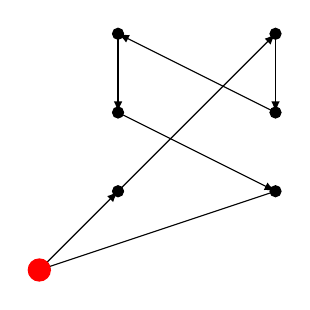
\begin{tikzpicture}
                \draw [black, -latex] (0, 0) -- (1, 1);
                \filldraw [black] (0, 0) circle (2pt);
                \draw [black, -latex] (1, 1) --(3, 3);
                \filldraw [black] (1, 1) circle (2pt);
                \draw [black, -latex] (3, 3) --(3, 2);
                \filldraw [black] (3, 3) circle (2pt);
                \draw [black, -latex] (3, 2) --(1, 3);
                \filldraw [black] (3, 2) circle (2pt);
                \draw [black, -latex] (1, 3) --(1, 2);
                \filldraw [black] (1, 3) circle (2pt);
                \draw [black, -latex] (1, 2) --(3, 1);
                \filldraw [black] (1, 2) circle (2pt);
                \draw [black, -latex] (3, 1) --(0, 0);
                \filldraw (3, 1) [black] circle (2pt);
                \filldraw [red] (0, 0) circle (4pt);
            \end{tikzpicture}
        \end{minipage}
        \begin{minipage}{0.3\linewidth}
            % Greedy
            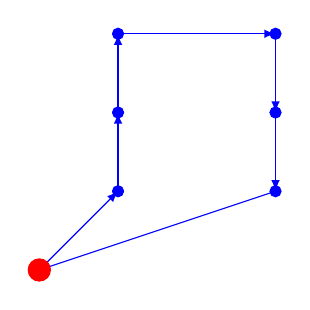
\begin{tikzpicture}
                \draw [blue, -latex] (0, 0) -- (1, 1);
                \filldraw [blue] (0, 0) circle (2pt);
                \draw [blue, -latex] (1, 1) --(1, 2);
                \filldraw [blue] (1, 1) circle (2pt);
                \draw [blue, -latex] (1, 2) --(1, 3);
                \filldraw [blue] (1, 2) circle (2pt);
                \draw [blue, -latex] (1, 3) --(3, 3);
                \filldraw [blue] (1, 3) circle (2pt);
                \draw [blue, -latex] (3, 3) --(3, 2);
                \filldraw [blue] (3, 3) circle (2pt);
                \draw [blue, -latex] (3, 2) --(3, 1);
                \filldraw [blue] (3, 2) circle (2pt);
                \draw [blue, -latex] (3, 1) --(0, 0);
                \filldraw (3, 1) [blue] circle (2pt);
                \filldraw [red] (0, 0) circle (4pt);
            \end{tikzpicture}
        \end{minipage}
        \begin{minipage}{0.3\linewidth}
            % opt2
            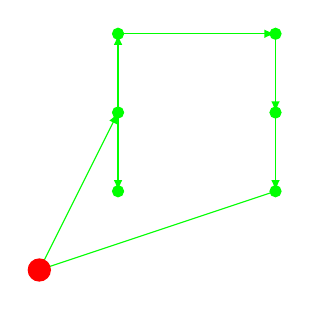
\begin{tikzpicture}
                \draw [green, -latex] (0, 0) -- (1, 2);
                \filldraw [green] (0, 0) circle (2pt);
                \draw [green, -latex] (1, 2) --(1, 1);
                \filldraw [green] (1, 2) circle (2pt);
                \draw [green, -latex] (1, 1) --(1, 3);
                \filldraw [green] (1, 1) circle (2pt);
                \draw [green, -latex] (1, 3) --(3, 3);
                \filldraw [green] (1, 3) circle (2pt);
                \draw [green, -latex] (3, 3) --(3, 2);
                \filldraw [green] (3, 3) circle (2pt);
                \draw [green, -latex] (3, 2) --(3, 1);
                \filldraw [green] (3, 2) circle (2pt);
                \draw [green, -latex] (3, 1) --(0, 0);
                \filldraw (3, 1) [green] circle (2pt);
                \filldraw [red] (0, 0) circle (4pt);
            \end{tikzpicture}
        \end{minipage}
    \end{figure}

    \subsection{Multiple Traveling Salesmen Problem}
    \label{subsection:Multiple_Traveling_Salesmen_Problem}
    Talk about how swap algorithm works. Figure \ref{figure:swapdemo} provides a simple example of how this algorithm improves the total distance. (Now prove it with data! What are the distances before and after?) ALSO: Talk about how the gray and black Addresses are symmetrical, but the trucks take different Routes. Is this okay, or does one or both of them need to go through greedy/opt2???

    \begin{figure}[h]
        \caption{Two Routes exchange Addresses to optimize their distances.}
        \label{figure:swapdemo}
        \begin{minipage}{0.45\linewidth}
            % Unswapped
            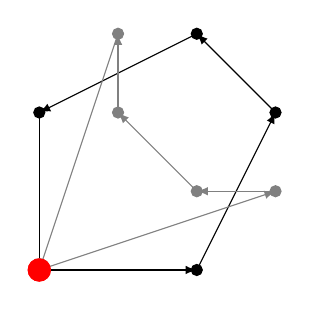
\begin{tikzpicture}
                % Route 1
                \draw [black, -latex] (0, 0) -- (2, 0);
                \filldraw [black] (0, 0) circle (2pt);
                \draw [black, -latex] (2, 0) --(3, 2);
                \filldraw [black] (2, 0) circle (2pt);
                \draw [black, -latex] (3, 2) --(2, 3);
                \filldraw [black] (3, 2) circle (2pt);
                \draw [black, -latex] (2, 3) --(0, 2);
                \filldraw [black] (2, 3) circle (2pt);
                \draw [black, -latex] (0, 2) --(0, 0);
                \filldraw (0, 2) [black] circle (2pt);
                \filldraw [red] (0, 0) circle (4pt);
                % Route 2
                \draw [gray, -latex] (0, 0) -- (3, 1);
                \filldraw [gray] (0, 0) circle (2pt);
                \draw [gray, -latex] (3, 1) --(2, 1);
                \filldraw [gray] (3, 1) circle (2pt);
                \draw [gray, -latex] (2, 1) --(1, 2);
                \filldraw [gray] (2, 1) circle (2pt);
                \draw [gray, -latex] (1, 2) --(1, 3);
                \filldraw [gray] (1, 2) circle (2pt);
                \draw [gray, -latex] (1, 3) --(0, 0);
                \filldraw (1, 3) [gray] circle (2pt);
                \filldraw [red] (0, 0) circle (4pt);
            \end{tikzpicture}
        \end{minipage}
        \begin{minipage}{0.45\linewidth}
            % Swapped
            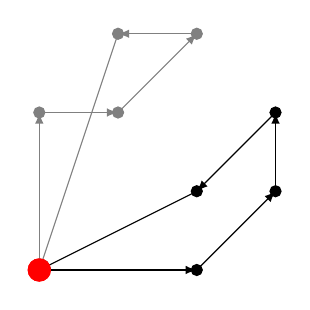
\begin{tikzpicture}
                % Route 1
                \draw [black, -latex] (0, 0) -- (2, 0);
                \filldraw [black] (0, 0) circle (2pt);
                \draw [black, -latex] (2, 0) --(3, 1);
                \filldraw [black] (2, 0) circle (2pt);
                \draw [black, -latex] (3, 1) --(3, 2);
                \filldraw [black] (3, 1) circle (2pt);
                \draw [black, -latex] (3, 2) --(2, 1);
                \filldraw [black] (3, 2) circle (2pt);
                \draw [black, -latex] (2, 1) --(0, 0);
                \filldraw (2, 1) [black] circle (2pt);
                \filldraw [red] (0, 0) circle (4pt);
                % Route 2
                \draw [gray, -latex] (0, 0) -- (0, 2);
                \filldraw [gray] (0, 0) circle (2pt);
                \draw [gray, -latex] (0, 2) --(1, 2);
                \filldraw [gray] (0, 2) circle (2pt);
                \draw [gray, -latex] (1, 2) --(2, 3);
                \filldraw [gray] (1, 2) circle (2pt);
                \draw [gray, -latex] (2, 3) --(1, 3);
                \filldraw [gray] (2, 3) circle (2pt);
                \draw [gray, -latex] (1, 3) --(0, 0);
                \filldraw (1, 3) [gray] circle (2pt);
                \filldraw [red] (0, 0) circle (4pt);
            \end{tikzpicture}
        \end{minipage}
    \end{figure}

    %%%%%
    %%%%%
    %%%%%
    %%%%% MORE DEVELOPMENT STEPS COULD GO HERE
    %%%%%
    %%%%%
    %%%%%

    \subsection{Developing the Final Product}
    \label{subsection:Developing_the_Final_Product}
    Our team 

    How is our final thing going to work? Basically we want it to work for businesses.

    \section{Results}
    \label{section:Results}
    Pretty pictures and tables go here. Describe each situation being displayed and talk about what they mean, e.g. is it the optimal solution? Good enough? Is there a tradeoff between time to execute and quality of results?

    Hmm, maybe insert a table comparing number of nodes/trucks to program execution time. What rate does it increase at $(O(n), O(n^2), \&c.)$

    \subsection{Scenario 1}

    \subsection{Scenario 2}

    \subsection{Performance Data}
    go over execution time and stuff

    \section{Conclusion}
    \label{section:Conclusion}
    Talk about what we learned, how this all applies to industry, ideas to scale the problem up, ethics, \&c.

    \appendix
    \section{Sample of Using Listings Package}
    Please remove this appendix before publishing! Here's some pretty C++ code from Listing \ref{lst:example}.
    \begin{lstlisting}[
        caption=Example Code,
        label={lst:example},
        language=C++
    ]
#include <iostream>
using sdt::cout;

int main() {
    // Print out hello
    cout << "Hello world!" << '\n';
    return 0;
}\end{lstlisting}
\end{document}